\chapter[Differential-Equation Based ABC's]{Differential-Equation
Based Absorbing Boundary Conditions \label{chap:abc}}

%\setcounter{page}{1}

\renewcommand{\thefootnote}{\fnsymbol{footnote}}
\footnotetext{Lecture notes by John Schneider.  {\tt
fdtd-abc.tex}}

\section{Introduction}

A simple absorbing boundary condition (ABC) was used in Chap.\
\ref{chap:fdtdIntro} to terminate the grid.  It relied upon the fact
that the fields were propagating in one dimension and the speed of
propagation was such that the fields moved one spatial step for every
time step, i.e., the Courant number was unity.  The node on the
boundary was updated using the value of the adjacent interior node
from the previous time step.  However, when a dielectric was
introduced, and the local speed of propagation was no longer equal to
$c$, this ABC ceased to work properly.  One would also find in higher
dimensions that this simple ABC would not work even in free space.
This is because the Courant number cannot be unity in higher
dimensions and this ABC does not account for fields which may be
obliquely incident on the edge of the grid.  The goal now is to find a
more general technique to terminate the grid.

Although the ABC we will discuss here is not considered
state-of-the-art, it provides a relatively simple way to terminate the
grid that is more than adequate in many circumstances.  Additionally,
some of the mathematical tools we will develop in this chapter can be
used in the analysis of a wide range of FDTD-related topics.

\section{The Advection Equation \label{sec:advection}}

The wave equation that governs the propagation of the electric field
in one dimension is
\begin{eqnarray}
  \frac{\partial^2 E_z}{\partial x^2}
  - \mu\epsilon \frac{\partial^2 E_z}{\partial t^2} &=& 0,
  \label{eq:waveEqOneD}
 \\
  \left(\frac{\partial^2}{\partial x^2}
  - \mu\epsilon \frac{\partial^2}{\partial t^2}\right) E_z &=& 0.
\end{eqnarray}
The second form represents the equation in terms of an operator
operating on $E_z$ where the operator is enclosed in parentheses.
This operator can be factored into the product of two operators and is
equivalent to
\begin{equation}
  \left(\frac{\partial }{\partial x}
  -\sqrt{\mu\epsilon} \frac{\partial }{\partial t}\right)
  \left(\frac{\partial }{\partial x}
  +\sqrt{\mu\epsilon} \frac{\partial }{\partial t}\right)
  E_z
  = 0.
  \label{eq:factoredWaveEq}
\end{equation}
Note that it does not matter which operator in
\refeq{eq:factoredWaveEq} is written first.  They commute and will
always ultimately yield \refeq{eq:waveEqOneD}.  If either of these
operators acting individually on the field yields zero, the wave
equation is automatically satisfied.  Thus an $E_z$ that satisfies
either of the following equations will also be a solution to the wave
equation:
\begin{eqnarray}
  \frac{\partial E_z}{\partial x}
  - \sqrt{\mu\epsilon} \frac{\partial E_z}{\partial t} &=& 0, 
  \label{eq:advection}
  \\
  \frac{\partial E_z}{\partial x}
  + \sqrt{\mu\epsilon} \frac{\partial E_z}{\partial t}
  &=& 0.
  \label{eq:advectionI}
\end{eqnarray}
These equations are sometimes called advection equations.  Note that a
solution to the wave equation will not simultaneously satisfy both
these advection equations (except in trivial cases).  It may satisfy
one or the other but not both.  In fact, fields may be a solution to
the wave equation and yet satisfy neither of the advection
equations.\footnote{As an example, consider $E_z(x,t) = \cos(\omega
  t)\sin(\beta x)$ where $\beta = \omega\sqrt{\mu\epsilon}$.}

A solution to \refeq{eq:advection} is
$E_z(t+\sqrt{\mu\epsilon}x)$, i.e., a wave traveling in the negative
$x$ direction.  The proof proceeds along the same lines
as the proof given in Sec.\ \ref{sec:waveEq}.  Equate the argument
with $\xi$ so that
\begin{equation}
  \xi = t+\sqrt{\mu\epsilon}x.
\end{equation}
Derivatives of the argument with respect to time or space are given by
\begin{equation}
  \frac{\partial\xi}{\partial t}=1  \quad \mbox{and} \quad
  \frac{\partial\xi}{\partial x}=\sqrt{\mu\epsilon}.
\end{equation}
Thus,
\begin{eqnarray}
 \frac{\partial E_z}{\partial x} \!&=&\!
    \frac{\partial E_z}{\partial \xi}\frac{\partial \xi}{\partial x} = 
    \sqrt{\mu\epsilon}\frac{\partial E_z}{\partial \xi}, 
 \label{eq:advecProof}
  \\
 \frac{\partial E_z}{\partial t} \!&=&\!
    \frac{\partial E_z}{\partial \xi}\frac{\partial \xi}{\partial t} = 
    \frac{\partial E_z}{\partial \xi}.
 \label{eq:advecProofI}
\end{eqnarray}
Plugging the right-hand sides of \refeq{eq:advecProof} and
\refeq{eq:advecProofI} into \refeq{eq:advection} yields zero and the
equation is satisfied.  It is worth mentioning that although
$E_z(t+\sqrt{\mu\epsilon}x)$ is a solution to 
\refeq{eq:advection}, it is not a solution to \refeq{eq:advectionI}.

\section{Terminating the Grid}

Let us now consider how an advection equation can be used to provide
an update equation for a node at the end of the computational domain.
Let the node $\fdtd{E_z}{0}{q+1}$ be the node on the boundary for
which an update equation is sought.  Since interior nodes can be
updated before the boundary node, assume that all the adjacent nodes
in space-time are known, i.e., $\fdtd{E_z}{1}{q+1}$,
$\fdtd{E_z}{0}{q}$, and $\fdtd{E_z}{1}{q}$ are known.  At the left end
of the grid, the fields should only be traveling to the left.  Thus
the fields satisfy the advection equation \refeq{eq:advection}.  The
finite-difference approximation of this equation provides the
necessary update equation, but the way to discretize the equation is
not entirely obvious.  A stable ABC will result if the equation is
expanded about the space-time point $(\Delx/2,(q+1/2)\Delt)$.  This
point is shown in Fig.\ \ref{fig:advectionABC}.

\begin{figure}
  \begin{center}
  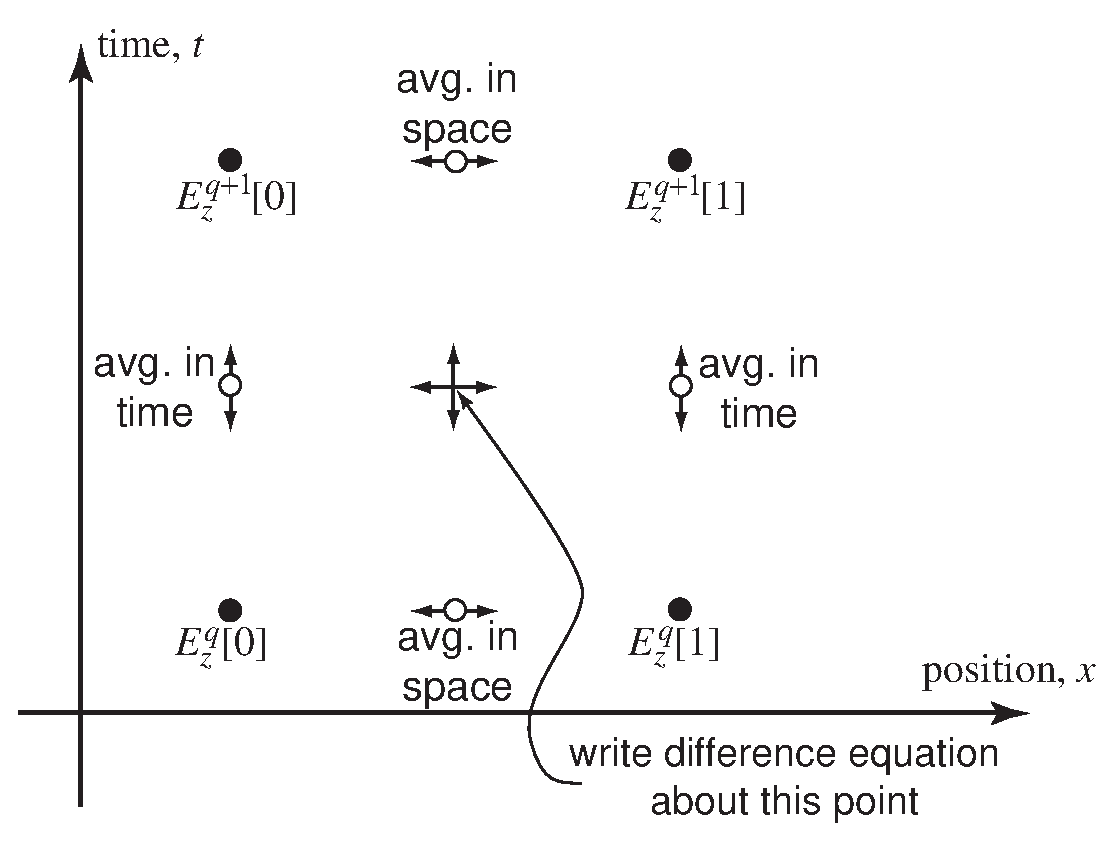
\epsfig{width=4.in,file=Figures/Fdtd-abc/abc-first-order.eps}
  \end{center}
  \caption{Space-time in the neighborhood of the left end of the grid.
  Only the electric fields are shown.  The open circles indicated
  where an electric field is needed for the advection equation.  Since
  there are none there, averaging is used to approximate the field at
  those points.}  \label{fig:advectionABC}
\end{figure}

At first it seems like this in an unacceptable point about which to
expand the advection equation since moving forward or backward in time
or space a half step does not correspond to the location of an
electric field point.  To fix this, the electric field will be averaged
in either time or space to obtain an estimate of the value at the
desired location in space-time.  For example, to obtain an
approximation of $\fdtd{E_z}{1/2}{q+1}$, the average
$(\fdtd{E_z}{0}{q+1}+\fdtd{E_z}{1}{q+1})/2$, would be used.
Similarly, an approximation of $\fdtd{E_z}{1/2}{q}$ would be
$(\fdtd{E_z}{0}{q}+\fdtd{E_z}{1}{q})/2$.  Therefore the temporal
derivative would be approximated with the following finite difference:
\begin{equation}
  \left. \sqrt{\mu\epsilon}
    \frac{\partial E_z}{\partial t}\right|_{\Delx/2,(q+1/2)\Delt}
  \approx
    \sqrt{\mu\epsilon}
    \frac{
     \frac{\fdtd{E_z}{0}{q+1}+\fdtd{E_z}{1}{q+1}}{2} -
     \frac{\fdtd{E_z}{0}{q}+\fdtd{E_z}{1}{q}}{2}
    }{\Delt}
   \label{eq:tDiffSpaceAvg}
\end{equation}

Averaging in time is used to obtain the fields at the proper locations
for the spatial finite difference.  The resulting finite difference is
\begin{equation}
  \left.
    \frac{\partial E_z}{\partial x}\right|_{\Delx/2,(q+1/2)\Delt}
  \approx
    \frac{
     \frac{\fdtd{E_z}{1}{q+1}+\fdtd{E_z}{1}{q}}{2} -
     \frac{\fdtd{E_z}{0}{q+1}+\fdtd{E_z}{0}{q}}{2}
    }{\Delx}
  \label{eq:xDiffTimeAvg}
\end{equation}
Combining \refeq{eq:tDiffSpaceAvg} and \refeq{eq:xDiffTimeAvg} yields
the finite-difference form of the advection equation
\begin{equation}
   \frac{
    \frac{\fdtd{E_z}{1}{q+1}+\fdtd{E_z}{1}{q}}{2} -
    \frac{\fdtd{E_z}{0}{q+1}+\fdtd{E_z}{0}{q}}{2}
   }{\Delx}
  -
   \sqrt{\mu\epsilon}
   \frac{
    \frac{\fdtd{E_z}{0}{q+1}+\fdtd{E_z}{1}{q+1}}{2} -
    \frac{\fdtd{E_z}{0}{q}+\fdtd{E_z}{1}{q}}{2}
   }{\Delt}
 = 0.
\end{equation}
Letting $\sqrt{\mu\epsilon}=\sqrt{\mu_r\epsilon_r}/c$ and
solving for $\fdtd{E_z}{0}{q+1}$ yields
\begin{equation}
  \fdtd{E_z}{0}{q+1} = \fdtd{E_z}{1}{q} +
    \frac{\frac{S_c}{\sqrt{\mu_r\epsilon_r}}-1}
         {\frac{S_c}{\sqrt{\mu_r\epsilon_r}}+1}
    \left(\fdtd{E_z}{1}{q+1}-\fdtd{E_z}{0}{q}\right)
  \label{eq:firstOrderABC}
\end{equation}
where $S_c$ is the Courant number $c\Delt/\Delx$.  Equation
\refeq{eq:firstOrderABC} provides a first-order absorbing boundary
condition that updates the field on the boundary using the values of
past and interior fields.  This is known as a first-order ABC because
it was constructed from a first-order differential equation.
Note that when $S_c/\sqrt{\mu_r\epsilon_r}$
is unity, which would be the case of free space and a unit Courant
number, \refeq{eq:firstOrderABC} reduces to $\fdtd{E_z}{0}{q+1} =
\fdtd{E_z}{1}{q}$ which is the simple grid-termination
technique presented in Sec.\ \ref{sec:terminate}.

At the other end of the grid, i.e., at the right end of the grid, an
equation that is nearly identical to \refeq{eq:firstOrderABC}
pertains.  Equation \refeq{eq:advectionI} would be expanded in the
neighborhood of the last node of the grid.  Although
\refeq{eq:advection} and \refeq{eq:advectionI} differ in the sign of
one term, when \refeq{eq:advectionI} is applied it is ``looking'' in
the negative $x$ direction.  That effectively cancels the sign change.
Hence the update equation for the last node in the grid, which is
identified here as $\fdtd{E_z}{M}{q+1}$, would be
\begin{equation}
  \fdtd{E_z}{M}{q+1} = \fdtd{E_z}{M-1}{q} +
    \frac{\frac{S_c}{\sqrt{\mu_r\epsilon_r}}-1}
         {\frac{S_c}{\sqrt{\mu_r\epsilon_r}}+1}
    \left(\fdtd{E_z}{M-1}{q+1}-\fdtd{E_z}{M}{q}\right).
  \label{eq:firstOrderABCI}
\end{equation}

Recall that for a lossless medium, the coefficient in the
electric-field update equation that multiplied the magnetic fields was
$\Delt/\epsilon\Delx$ and this could be expressed as
$S_c\eta_0/\epsilon_r$.  On the other hand, the coefficient in the
magnetic-field update equation that multiplied the electric fields was
$\Delt/\mu\Delx$ and this could be expressed as $S_c/\eta_0\mu_r$.
Therefore, taking the product of these two coefficients and taking the
square root yields
\begin{equation}
  \left(\frac{\Delt}{\epsilon\Delx}
        \frac{\Delt}{\mu\Delx}\right)^{1/2} =
        \frac{S_c}{\sqrt{\mu_r\epsilon_r}}.
  \label{eq:abcCoefFirstOrder}
\end{equation}
Note that this is the term that appears in \refeq{eq:firstOrderABC}
and \refeq{eq:firstOrderABCI}.
Thus by knowing the update coefficients that pertain at the ends of
the grid, one can calculate the coefficients that appear in the ABC.

\section{Implementation of a First-Order ABC}

Program \ref{pro:1Ddielectric} modeled two half spaces: free space and
a dielectric.  That program was written as a ``monolithic'' program
with a {\tt main()} function in which all the calculations were
performed.  For that program we did not have a suitable way to
terminate the grid within the dielectric.  Let us re-implement that
program but use the modular design that was discussed in Chap.\
\ref{chap:fdtdImproved} and use the ABC presented in the previous
section.  

Recalling the modular design used to model a lossy layer that was
discussed in Sec.\ \ref{sec:improveThree}, we saw that the ABC was so
simple there was no need to do any initialization of the ABC.
Nevertheless, recalling the code shown in Program \ref{pro:improved3},
an ABC initialization function was called, but it merely returned
without doing anything.  Now that we wish to implement a first-order
ABC, the ABC initialization function actually needs to perform some
calculations: it will calculate any of the constants associated with
the ABC.  

Naturally, the code associated with the various
``blocks'' in our modular design will need to change from what was
presented in Sec.\ \ref{sec:improveThree}.  However, the overall
framework remains essentially the same!  The arrangement of files
associated with our model of halfspace that uses a first-order ABC
is shown in Fig.\ \ref{fig:firstOrderAbcFiles}.  Note that this figure
and Fig.\ \ref{fig:improvedFiles} are nearly the same.  They both have
the same layout.  All the functions have the same name, but the
implementation of some of those functions have changed.  Note that the
file names have changed for the files containing the {\tt main()}
function, the {\tt gridInit()} function, and the {\tt abc()} and {\tt
  abcInit()} function.  
\begin{figure}
  \begin{center}
  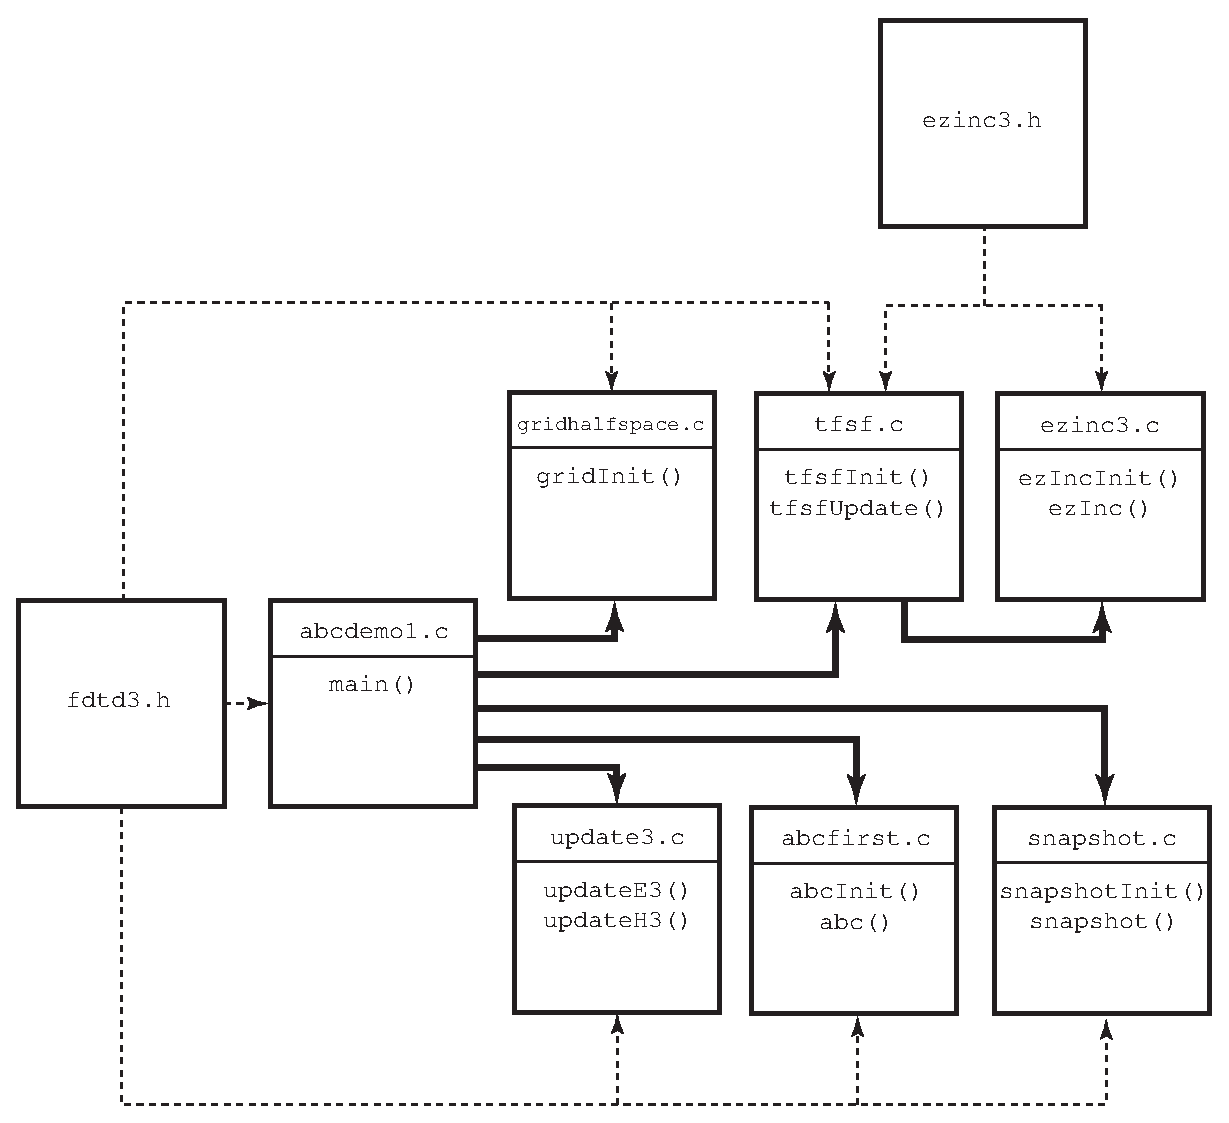
\epsfig{width=6.3in,file=Figures/Fdtd-abc/abcdemo1-files.eps}
\end{center} \caption{Files associated with the modular implementation
  of a simulation of a dielectric half space.  Since a first-order ABC
  is now being used, some of these files differ from those of Fig.\
  \ref{fig:improvedFiles}.  Nevertheless, the overall structure of the
  program is unchanged and all the function names are the same as
  before.}
  \label{fig:firstOrderAbcFiles}
\end{figure}


The code associated with the TFSF boundary, the snapshots, the source
function, and the update equations are all unchanged from that which
was described in Chap.\ \ref{chap:fdtdImproved}.  The grid
initialization function {\tt gridInit()} constructs a half-space
dielectric consistent with Program \ref{pro:1Ddielectric}.  The code
is shown in Program \ref{pro:gridInit1DhalfSpace}.

\begin{program} {\tt gridhalfspace.c}: Function to initialize the {\tt
    Grid} such that there are two half-spaces: free space to the left
  and a dielectric with $\epsilon_r=9$ to the right.
\label{pro:gridInit1DhalfSpace}
\codemiddle
\begin{lstlisting}
/* Function to initialize the Grid structure. */

#include "fdtd3.h"

#define EPSR 9.0

void gridInit(Grid *g) {
  double imp0 = 377.0;
  int mm;

  SizeX = 200;   // size of domain
  MaxTime = 450; // duration of simulation
  Cdtds = 1.0;   // Courant number

  ALLOC_1D(g->ez,   SizeX, double);
  ALLOC_1D(g->ceze, SizeX, double);
  ALLOC_1D(g->cezh, SizeX, double);
  ALLOC_1D(g->hy,   SizeX - 1, double);
  ALLOC_1D(g->chyh, SizeX - 1, double);
  ALLOC_1D(g->chye, SizeX - 1, double);
  
  /* set electric-field update coefficients */
  for (mm = 0; mm < SizeX; mm++)
    if (mm < 100) {
      Ceze(mm) = 1.0;
      Cezh(mm) = imp0;
    } else {
      Ceze(mm) = 1.0;
      Cezh(mm) = imp0 / EPSR;
    }

  /* set magnetic-field update coefficients */
  for (mm = 0; mm < SizeX - 1; mm++) {
    Chyh(mm) = 1.0;
    Chye(mm) = 1.0 / imp0;
  }

  return;
}
\end{lstlisting}
\end{program}

The contents of the file {\tt abcdemo1.c} are shown in Program
\ref{pro:abcdemo1}.  The difference between {\tt abcdemo1.c} and {\tt
  improved3.c}, which is given in Program \ref{pro:improved3}, is
shown in bold.  In fact, the only change in the code is the location of
the call of the ABC function {\tt abc()}.  Function {\tt abc()} is now
called in line \ref{abcdemo1B} which is {\em after} the updating of
the electric fields.  Since the ABC relies on the ``future'' value of
a neighboring interior electric field, this field must be updated
before the node on the grid boundary can be updated.  (The ABC
function presented in Program \ref{pro:improved3} could, in fact, have
been written in such a way that it would be called after the
electric-field update.  After all, the first-order ABC reduces to the
simple ABC when the Courant number is one and the medium is free
space.  Nevertheless, the code in Program \ref{pro:improved3} was
written to be consistent with the way in which the simple ABC was
originally presented in Chap.\ \ref{chap:fdtdIntro}.)

\begin{program}
{\tt abcdemo1.c}: One-dimensional FDTD simulation employing a
first-order ABC (although the actual ABC code is contained in the
file {\tt abcfirst.c} which is shown in Program \ref{pro:abcfirst}).
The difference between this program and Program \ref{pro:improved3}
is shown in bold.
\label{pro:abcdemo1}
\codemiddle
\begin{lstlisting}
/* FDTD simulation where main() is primarily used to call other
 * functions that perform the necessary operations. */

#include "fdtd3.h"

int main()
{
  Grid *g;

  ALLOC_1D(g, 1, Grid);  // allocate memory for Grid

  gridInit(g);         // initialize the grid
  abcInit(g);          // initialize ABC  /*@ \label{abcdemo1A} @*/
  tfsfInit(g);         // initialize TFSF boundary
  snapshotInit(g);     // initialize snapshots

  /* do time stepping */
  for (Time = 0; Time < MaxTime; Time++) {

    updateH3(g);   // update magnetic field
    tfsfUpdate(g); // correct field on TFSF boundary
    updateE3(g);   // update electric field
/*b*/    abc(g);/*n*/         // apply ABC -- after E-field update/*@ \label{abcdemo1B} @*/
    snapshot(g);   // take a snapshot (if appropriate)

  } /* end of time-stepping */

  return 0;
}
\end{lstlisting}
\end{program}

The code for {\tt abcInit()} and {\tt abc()} is contained in the file
{\tt abcfirst.c} which is shown in Program \ref{pro:abcfirst}.  The
initialization function calculates the coefficients that appeared in
\refeq{eq:firstOrderABC} and \refeq{eq:firstOrderABCI}.  Recall from
\refeq{eq:abcCoefFirstOrder} that these coefficients can be obtained as
a function of the electric- and magnetic-field update-equation
coefficients.  Since the material at the left and right side of the
grid may be different, there are separate coefficients for the two
sides.

\begin{program}
{\tt abcfirst.c}: Implementation of a first-order absorbing boundary
condition. 
\label{pro:abcfirst}
\codemiddle
\begin{lstlisting}
/* Function to implement a first-order ABC. */

#include "fdtd3.h"
#include <math.h>

static int initDone = 0;
static double ezOldLeft = 0.0, ezOldRight = 0.0;
static double abcCoefLeft, abcCoefRight;

/* Initizalization function for first-order ABC. */
void abcInit(Grid *g) {
  double temp;
  
  initDone = 1;

  /* calculate coefficient on left end of grid */
  temp = sqrt(Cezh(0) * Chye(0));
  abcCoefLeft = (temp - 1.0) / (temp + 1.0);

  /* calculate coefficient on right end of grid */
  temp = sqrt(Cezh(SizeX - 1) * Chye(SizeX - 2));
  abcCoefRight = (temp - 1.0) / (temp + 1.0);

  return;
}

/* First-order ABC. */
void abc(Grid *g) {
  /* check if abcInit() has been called */
  if (!initDone) {
    fprintf(stderr,
	    "abc: abcInit must be called before abc.\n");
    exit(-1);
  }

  /* ABC for left side of grid */
  Ez(0) = ezOldLeft + abcCoefLeft * (Ez(1) - Ez(0));
  ezOldLeft = Ez(1);  /*@ \label{abcfirstA} @*/

  /* ABC for right side of grid */
  Ez(SizeX - 1) = ezOldRight + 
    abcCoefRight * (Ez(SizeX - 2) - Ez(SizeX - 1));
  ezOldRight = Ez(SizeX - 2);  /*@ \label{abcfirstB} @*/

  return;
}
\end{lstlisting}
\end{program}

As shown in \refeq{eq:firstOrderABC} and \refeq{eq:firstOrderABCI},
for the first-order ABC both the ``past'' and the future value of the
interior neighbor nearest to the boundary are needed.  However, once
we update the fields, past values are overwritten.  Thus, the function
{\tt abc()}, which applies the ABC to the two ends of the grid,
locally stores the ``past'' values of the nodes that are adjacent to
the ends of the grid.  For the left side of the grid the past neighbor
is stored as {\tt ezOldLeft} and on the right it is stored as {\tt
  ezOldRight}.  These are static global variables that are retained
from one invocation of {\tt abc()} to the next.  Thus, even though the
interior fields have been updated, these past values will still be
available.  (Once the nodes at the ends of the grid have been updated,
{\tt ezOldLeft} and {\tt ezOldRight} are set to the current value of
the neighboring nodes as shown in lines \ref{abcfirstA} and
\ref{abcfirstB}.  When {\tt abc()} is called next, these are indeed
the ``old'' values of these neighbors.)

Figure \ref{fig:dielectricABC} shows the waterfall plot of the
snapshots generated by Program \ref{pro:abcdemo1}.  One can see that
this is the same as Fig.\ \ref{fig:waterfallDielec} prior to the
transmitted field encountering the right end of the grid.  After that
time there is a reflected field evident in Fig.\
\ref{fig:waterfallDielec} but none is visible here.  The ABC has
absorbed the incident field and hence the grid behaves as if it were
infinite.  In reality this ABC is only approximate and there is some
reflected field at the right boundary.  We will return to this point
in Sec. \ref{sec:secondOrderABC}

\begin{figure}
  \begin{center}
  \epsfig{width=4.6in,file=Code/Fdtd-abc/waterfall-die-abc.eps}
  \end{center}
  \caption{Waterfall plot of the snapshots generated by Program
  \ref{pro:abcdemo1}.  Comparing this to Fig.\
  \ref{fig:waterfallDielec} one sees they are the same until the transmitted
  field encounters the right end of the grid.  At that point
  \ref{fig:waterfallDielec} shows there is a reflected field.  However,
  because of the ABC used here, no reflected field is visible.}
  \label{fig:dielectricABC}
\end{figure}

\section{ABC Expressed Using Operator Notation \label{sec:abcOperator}}

Let us define an identity operator $I$, a forward spatial shift
operator $s_x^{1}$, and a backward temporal shift operator $s_t^{-1}$.
When they act on a node in the grid their affect is given by
\begin{eqnarray}
  I\fdtd{E_z}{m}{q+1} &=& \fdtd{E_z}{m}{q+1}, \\
  s_x^{1}\fdtd{E_z}{m}{q+1} &=& \fdtd{E_z}{m+1}{q+1}, \\
  s_t^{-1}\fdtd{E_z}{m}{q+1} &=& \fdtd{E_z}{m}{q}.
\end{eqnarray}
Note that these operators all commute, e.g., $s_x^{1}s_t^{-1} =
s_t^{-1}s_x^{1}$.  Furthermore, the identity operator times another
operator is merely that operator, e.g., $Is_x^{1} = s_x^{1}$ likewise
$II = I$.  Using these operators a spatial average of a node can be
represented by
\begin{equation}
  \frac{\fdtd{E_z}{m}{q+1} + \fdtd{E_z}{m+1}{q+1}}{2} =
  \left(\frac{I+s_x^{1}}{2}\right)\fdtd{E_z}{m}{q+1},
\end{equation}
while a temporal average can be written
\begin{equation}
  \frac{\fdtd{E_z}{m}{q+1} + \fdtd{E_z}{m}{q}}{2} =
  \left(\frac{I+s_t^{-1}}{2}\right)\fdtd{E_z}{m}{q+1}.
\end{equation}

When applying the advection equation, the finite differences, as
originally formulated, needed electric-field nodes where none were
present in space-time.  Therefore, averaging had to be used to obtain
approximations to the fields at the desired locations.  This required
averaging in time followed by a spatial finite difference or averaging
in space followed by a temporal finite difference.  Consider the
finite difference approximation to the temporal derivative at the
point $(\Delx/2,(q+1/2)\Delt)$.  Starting from the node
$\fdtd{E_z}{0}{q+1}$, this requires adding the node one spatial step
to the right and then dividing by two.  Then, going back one step in
time, these same two nodes are again averaged and then subtracted from
the previous average.  The result is divided by the temporal step to
obtain the temporal finite difference.  Expressed in operator notation
this is
\begin{eqnarray}
  \left.\frac{\partial E_z}{\partial t}\right|_{\Delx/2,(q+1/2)\Delt}
  &=& 
    \left(\frac{I-s_t^{-1}}{\Delt}\right)
    \left(\frac{I+s_x^{1}}{2}\right)\fdtd{E_z}{0}{q+1} 
    \label{eq:operatorDetails}
 \\
  &=&
    \frac{1}{2\Delt}
    \left(I - s_t^{-1} + s_x^{1} - s_t^{-1}s_x^{1}\right)\fdtd{E_z}{0}{q+1} \\
  &=&
    \frac{1}{2\Delt}
    \left(\fdtd{E_z}{0}{q+1} - \fdtd{E_z}{0}{q}
        + \fdtd{E_z}{1}{q+1} - \fdtd{E_z}{1}{q}\right).
    \label{eq:operatorDetailsII}
\end{eqnarray}
The second term in parentheses in \refeq{eq:operatorDetails}
accomplishes the averaging while the first term in parentheses yields
the temporal finite difference.  The result, shown in
\refeq{eq:operatorDetailsII}, is the same as \refeq{eq:tDiffSpaceAvg}
(other than the factor of $\sqrt{\mu\epsilon}$).

A similar approach can be used for the spatial finite difference about
the same point except now the averaging is done in time
\begin{eqnarray}
  \left.\frac{\partial E_z}{\partial x}\right|_{\Delx/2,(q+1/2)\Delt}
  &=& 
    \left(\frac{s_x^{1}-I}{\Delx}\right)
    \left(\frac{I+s_t^{-1}}{2}\right)\fdtd{E_z}{0}{q+1} 
    \label{eq:operatorDetailsIII}
 \\
  &=&
    \frac{1}{2\Delx}
    \left(-I + s_x^{1} - s_t^{-1} + s_t^{-1}s_x^{1}\right)\fdtd{E_z}{0}{q+1} \\
  &=&
    \frac{1}{2\Delx}
    \left(-\fdtd{E_z}{0}{q+1} + \fdtd{E_z}{1}{q+1}
        - \fdtd{E_z}{0}{q} + \fdtd{E_z}{1}{q}\right).
\end{eqnarray}
This is exactly the same as \refeq{eq:xDiffTimeAvg}.

From \refeq{eq:operatorDetails} and \refeq{eq:operatorDetailsIII} we
see the finite-difference form of the advection equation can be
expressed as
\begin{equation}
   \left\{\left(\frac{s_x^{1}-I}{\Delx}\right)
         \left(\frac{I+s_t^{-1}}{2}\right) -
    \sqrt{\mu\epsilon}
    \left(\frac{I-s_t^{-1}}{\Delt}\right)
    \left(\frac{I+s_x^{1}}{2}\right)\right\}
    \fdtd{E_z}{0}{q+1} = 0.
   \label{eq:advectionOperator}
\end{equation}
Solving this equation for $\fdtd{E_z}{0}{q+1}$ yields the update
equation \refeq{eq:firstOrderABC}.  The term in braces is the
finite-difference equivalent of the first advection operator that
appeared on the left-hand side of \refeq{eq:factoredWaveEq}.

\section{Second-Order ABC \label{sec:secondOrderABC}}

Equation \refeq{eq:advectionOperator} provides an update equation
which is, in general, approximate.  In many circumstance the field
reflected by a first-order ABC is unacceptably large.  A more accurate
update equation can be obtained by applying the advection operator
twice.  Consider 
\begin{equation}
  \left(\frac{\partial }{\partial x}
  -\sqrt{\mu\epsilon} \frac{\partial }{\partial t}\right)
  \left(\frac{\partial }{\partial x}
  -\sqrt{\mu\epsilon} \frac{\partial }{\partial t}\right)
  E_z
  = 0.
  \label{eq:advectionSecond}
\end{equation}
Without employing too many mathematical details, assume the field
$E_z$ is not a proper solution to the advection equation.  For
example, the speed at which it is propagating is not precisely
$1/\sqrt{\mu\epsilon}$.  If the field is close to a proper solution,
the advection operator operating on the field should yield a number
which is close to zero.  However, if the advection operator acts on it
again, the result should be something smaller still---the equation is
closer to the truth.  

To demonstrate this, consider a wave $E_z(t+x/c')$ which is traveling
in the negative $x$ direction with a speed $c'\neq c$.  Following the
notation used in Sec.\ \ref{sec:advection}, the advection operator
operating on this fields yields
\begin{equation}
  \left(\frac{1}{c'} - \frac{1}{c}\right)
  \frac{\partial E_z}{\partial \xi}.
  \label{eq:advectionResidue}
\end{equation}
If the advection operator again operates on this, the result is
\begin{equation}
  \left(\frac{1}{c'} - \frac{1}{c}\right)^2
  \frac{\partial^2 E_z}{\partial \xi^2}.
  \label{eq:advectionResidueI}
\end{equation}
If $c$ and $c'$ are close, \refeq{eq:advectionResidueI} will be smaller
than \refeq{eq:advectionResidue} for a broad class of signals.  Hence
the repeated application of the advection operator may still only be
approximately satisfied, but one anticipates that it will perform
better than the first-order operator alone.

The finite-difference form of the second-order advection operator
operating on the node $\fdtd{E_z}{0}{q+1}$ is
\begin{eqnarray}
   \left[\left\{\left(\frac{s_x^{1}-I}{\Delx}\right)
         \left(\frac{I+s_t^{-1}}{2}\right) -
    \sqrt{\mu\epsilon}
    \left(\frac{I-s_t^{-1}}{\Delt}\right)
    \left(\frac{I+s_x^{1}}{2}\right)\right\}\right.\qquad\qquad\mbox{ }&& 
   \nonumber\\
   \left.\left\{\left(\frac{s_x^{1}-I}{\Delx}\right)
         \left(\frac{I+s_t^{-1}}{2}\right) -
    \sqrt{\mu\epsilon}
    \left(\frac{I-s_t^{-1}}{\Delt}\right)
    \left(\frac{I+s_x^{1}}{2}\right)\right\}\right]
    \fdtd{E_z}{0}{q+1} &=& 0.
   \label{eq:advectionOperatorI}
\end{eqnarray}
One expands this equation and solves for $\fdtd{E_z}{0}{q+1}$ to
obtain the second-order ABC.  The result is
\begin{eqnarray}
  \fdtd{E_z}{0}{q+1} &=& \frac{-1}{1/S_c'+2+S_c'}
   \left\{(1/S_c'-2+S_c')
   \left[\fdtd{E_z}{2}{q+1}+\fdtd{E_z}{0}{q-1}\right]\right. \nonumber\\
  && \hspace{.4in}\mbox{}+2(S_c'-1/S_c')
  \left[\fdtd{E_z}{0}{q} + \fdtd{E_z}{2}{q} 
        - \fdtd{E_z}{1}{q+1}-\fdtd{E_z}{1}{q-1}\right] \nonumber\\
  &&
  \left.\hspace{1.5in}\mbox{}-4(1/S_c'+S_c')\fdtd{E_z}{1}{q}\right\}
   - \fdtd{E_z}{2}{q-1}
  \label{eq:secondOrderABC}
\end{eqnarray}
where
$S_c'=\Delt/(\sqrt{\mu\epsilon}\Delx)=S_c/\sqrt{\mu_r\epsilon_r}$.
This update equation requires two interior points at time step $q+1$
as well as the boundary node and these same interior points at time
steps $q$ and $q-1$.  Typically these past values would not be
available to use in the update equation and must therefore be stored
in some auxiliary manner such as had to be done in Program
\ref{pro:abcfirst} (there just a single point on either end of
the grid needed to be stored).  Two $3\times 2$ arrays (one used at
either end of the computational domain) could be used to store the
values at the three spatial locations and two previous time steps
required by \refeq{eq:secondOrderABC}.  Alternatively, four 1D arrays
(two used at either end) of three points each could also be used to
stored the old values.  (It may be noted that $\fdtd{E_z}{0}{q}$ would
not need to be stored since it would be available when updating the
boundary node.  However, for the sake of symmetry when writing the
loops which store the boundary values, it is simplest to store this
value explicitly.)

When $S_c'$ is unity, as would be the case for propagation in free space
with a Courant number of unity, \refeq{eq:secondOrderABC} reduces to
\begin{equation}
  \fdtd{E_z}{0}{q+1} = 2\fdtd{E_z}{1}{q} - \fdtd{E_z}{2}{q-1}.
\end{equation}
This may appear odd at first but keep in mind that the field is only
traveling to the left and it moves one spatial step per time step,
thus $\fdtd{E_z}{1}{q}$ and $\fdtd{E_z}{2}{q-1}$ are equal.  Therefore
this effectively reduces to $\fdtd{E_z}{0}{q+1} = \fdtd{E_z}{1}{q}$
which is again the original grid termination approach used in Sec.\
\ref{sec:terminate}.

As was the case for first-order, for the right side of the grid, the
second-order termination is essentially the same as the one on the
left side.  One merely uses interior nodes to the left of the boundary
instead of to the right.

To demonstrate the improvement realized by using a second-order ABC
instead of a first-order one, consider the same computational domain
as was used in Program \ref{pro:abcdemo1}, i.e., a pulse is
incident from free space to a dielectric half-space with a relative
permittivity of $9$ which begins at node $100$.  Figure
\ref{fig:firstSecondABC} shows the electric field in the
computational domain at time-step $550$ ({\tt MaxTime} was increased
from the $450$ shown in Program \ref{pro:gridInit1DhalfSpace}).
Ideally the transmitted pulse would be perfectly absorbed and the
reflected fields should be zero.  However, for both the first- and
second-order ABC's there is a reflected field, but it is significantly
smaller in the case of the second-order ABC.

\begin{figure}
  \begin{center}
  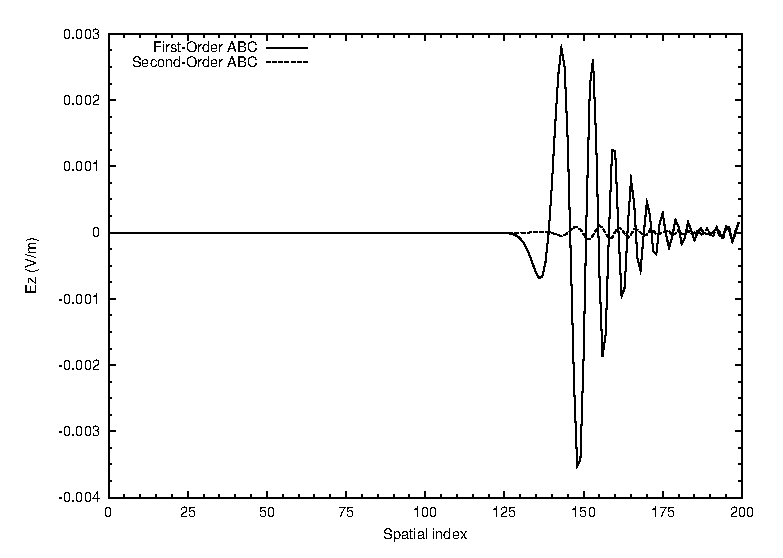
\epsfig{width=4.5in,file=Code/Fdtd-abc/abc-first-second.eps}
  \end{center}
  \caption{Plot of the fields at time step 550 when the grid is
  terminated with either a first- or second-order ABC.  This snapshot
  is taken after the transmitted pulse has encountered the right edge of
  the grid.  Hence this shows the field reflected by the ABC.  Ideally the
  reflected fields should be zero.}
  \label{fig:firstSecondABC}
\end{figure}

\newpage

\section{Implementation of a Second-Order ABC
  \label{sec:secondAbc}}

In order to implement a second-order ABC, one merely has to modify the
functions {\tt abcInit()} and {\tt abc()}.  Thus, none of the code
depicted in Fig.\ \ref{fig:firstOrderAbcFiles} needs to change except
for that which is directly related to the ABC itself.  If instead of
using the file {\tt abcfirst.c}, one uses the code shown in Program
\ref{pro:abcsecond}, which we assume is stored in a file called {\tt
abcsecond.c}, then a second-order ABC will be realized.

\begin{program}
{\tt abcsecond.c} The {\tt abcInit()} and {\tt abc()} functions for
implementation of a second-orde ABC.
\label{pro:abcsecond}
\codemiddle
\begin{lstlisting}
/* Functions to implement a second-order ABC. */

#include "fdtd3.h"
#include <math.h>

static int initDone = 0;
static double *ezOldLeft1, *ezOldLeft2, /*@ \label{abcsecondA} @*/
              *ezOldRight1, *ezOldRight2;
static double *abcCoefLeft, *abcCoefRight; /*@ \label{abcsecondB} @*/

/* Initizalization function for second-order ABC. */
void abcInit(Grid *g) {
  double temp1, temp2;
  
  initDone = 1;

  ALLOC_1D(ezOldLeft1, 3, double); /*@ \label{abcsecondC} @*/
  ALLOC_1D(ezOldLeft2, 3, double);
  ALLOC_1D(ezOldRight1, 3, double);
  ALLOC_1D(ezOldRight2, 3, double);

  ALLOC_1D(abcCoefLeft, 3, double);
  ALLOC_1D(abcCoefRight, 3, double); /*@ \label{abcsecondD} @*/

  /* calculate coefficients on left end of grid */
  temp1 = sqrt(Cezh(0) * Chye(0));
  temp2 = 1.0 / temp1 + 2.0 + temp1;
  abcCoefLeft[0] = -(1.0 / temp1 - 2.0 + temp1) / temp2;
  abcCoefLeft[1] = -2.0 * (temp1 - 1.0 / temp1) / temp2;
  abcCoefLeft[2] = 4.0 * (temp1 + 1.0 / temp1) / temp2;

  /* calculate coefficients on right end of grid */
  temp1 = sqrt(Cezh(SizeX - 1) * Chye(SizeX - 2));
  temp2 = 1.0 / temp1 + 2.0 + temp1;
  abcCoefRight[0] = -(1.0 / temp1 - 2.0 + temp1) / temp2;
  abcCoefRight[1] = -2.0 * (temp1 - 1.0 / temp1) / temp2;
  abcCoefRight[2] = 4.0 * (temp1 + 1.0 / temp1) / temp2;

  return;
}

/* Second-order ABC. */
void abc(Grid *g) {
  int mm;

  /* check if abcInit() has been called */
  if (!initDone) {
    fprintf(stderr,
	    "abc: abcInit must be called before abc.\n");
    exit(-1);
  }

  /* ABC for left side of grid */
  Ez(0) = abcCoefLeft[0] * (Ez(2) + ezOldLeft2[0]) /*@ \label{abcsecondE} @*/
    + abcCoefLeft[1] * (ezOldLeft1[0] + ezOldLeft1[2] -
		        Ez(1) - ezOldLeft2[1])
    + abcCoefLeft[2] * ezOldLeft1[1] - ezOldLeft2[2];

  /* ABC for right side of grid */
  Ez(SizeX-1) =  /*@ \label{abcsecondF} @*/
    abcCoefRight[0] * (Ez(SizeX - 3) + ezOldRight2[0])
    + abcCoefRight[1] * (ezOldRight1[0] + ezOldRight1[2] -
		         Ez(SizeX - 2) - ezOldRight2[1])
    + abcCoefRight[2] * ezOldRight1[1] - ezOldRight2[2];

  /* update stored fields */
  for (mm = 0; mm < 3; mm++) {  /*@ \label{abcsecondG} @*/
    ezOldLeft2[mm] = ezOldLeft1[mm];
    ezOldLeft1[mm] = Ez(mm);
    
    ezOldRight2[mm] = ezOldRight1[mm];
    ezOldRight1[mm] = Ez(SizeX - 1 - mm);
  }

  return;
}
\end{lstlisting}
\end{program}

Lines \ref{abcsecondA}--\ref{abcsecondB} declare six static, global
pointers, each of which will ultimately serve as an array of three
points.  Four of the arrays will store previous values of the electric
field (two arrays dedicated to the left side and two to the right).
The remaining two arrays store the coefficients used in the ABC (one
array for the left, one for the right).  The memory for these arrays
is allocated in the {\tt abcInit()} function in lines
\ref{abcsecondC}--\ref{abcsecondD}.  That is followed by calculation
of the coefficients on the two side of the grid.

Within the function {\tt abc()}, which is called once per time-step,
the values of the nodes on the edge of the grid are updated by the
statements starting on lines
\ref{abcsecondE} and \ref{abcsecondF}.  Finally, starting on line
\ref{abcsecondG}, the stored values are updated.  The array {\tt
exOldLeft1} represents the field one time-step in the past while 
{\tt exOldLeft2} represents the field two time-steps in the past.
Similar naming is employed on the right.
